\documentclass[conference]{IEEEtran}
% Compile on Overleaf with pdfLaTeX + BibTeX. Upload main.tex, refs.bib, figures/*.pdf.

\usepackage{amsmath,amssymb}
\usepackage{graphicx}
\usepackage{booktabs}
\usepackage{multirow}
\usepackage{xcolor}
\usepackage{url}
\usepackage[hidelinks]{hyperref}

% Anything inside \pending{} is waiting on Run C and must be filled before submission.
\newcommand{\pending}[1]{\textcolor{red}{[PENDING: #1]}}
\newcommand{\stask}{S_{\text{task}}}
\newcommand{\sgen}{S_{\text{gen}}}
\newcommand{\slt}{S_{\text{L2}}}
\newcommand{\sUp}{S_{\text{up}}}

\begin{document}

\title{Is 4-Bit Enough? Signal-Gated Evaluation of Quantized\\LLM Vulnerability Detectors}

\author{
\IEEEauthorblockN{Siddhant Singh}
\IEEEauthorblockA{School of Computer Science and Engineering\\
Vellore Institute of Technology, Vellore, India\\
siddhant3103@gmail.com}
\and
\IEEEauthorblockN{Gunavathi C}
\IEEEauthorblockA{School of Computer Science and Engineering\\
Vellore Institute of Technology, Vellore, India\\
\textcolor{red}{[guide's email]}}
}

\maketitle

\begin{abstract}
Small open code LLMs are attractive as on-premise security auditors, and weight quantization is the standard way to fit them on commodity GPUs. Prior work on mixed-precision quantization argues that ``sensitive'' layers should keep more bits. We ask whether this matters for LLM-based vulnerability detection, and find that the answer depends on an evaluation step that is usually skipped: checking that the full-precision model has any detection signal at all. Across four models and three benchmarks, we find that (i)~on PrimeVul paired data every model up to 8B parameters is at chance in FP16, so quantization comparisons there are uninformative and can even show spurious ``improvements''; (ii)~on the Juliet suite, lexical cues (function names such as \texttt{bad}/\texttt{good} and \texttt{FLAW} comments) inflate FP16 AUROC from 0.68 to 0.98, and removing them is essential; (iii)~where signal exists, uniform 4-bit and even 3-bit quantization are statistically equivalent to FP16 within $\pm$0.02 AUROC at 34--38\% of the weight memory, and sensitivity-guided INT8/NF4 mixtures add nothing; (iv)~below that, quality collapses, and the collapse point depends on model size: 2 bits for the 7B model, 3 bits for the 3B model, where it stops answering YES/NO at all; (v)~at 2 bits, which layers keep 4 bits moves AUROC by 0.06 at identical memory, yet none of four layer-sensitivity metrics, including a new deployment-context ``upgrade'' metric, beats random selection, and depth-correlated metrics pick the worst layers. We also show that quantization shifts score calibration far more than ranking, so fixed-threshold metrics are misleading. We release code, cleaned splits and all per-function predictions.
\end{abstract}

\begin{IEEEkeywords}
vulnerability detection, large language models, quantization, mixed precision, benchmark leakage, evaluation methodology
\end{IEEEkeywords}

%=====================================================================
\section{Introduction}
%=====================================================================
Code-specialised LLMs are increasingly proposed as automated security auditors~\cite{ullah2024secllmholmes,ding2024primevul}. For many organisations, source code cannot leave the premises, which favours small open models (3--8B parameters) run locally. Even these do not fit comfortably on commodity GPUs in FP16: Qwen2.5-Coder-7B needs 14.2\,GB of weights. Post-training weight quantization (8-bit~\cite{dettmers2022llmint8}, 4-bit NF4~\cite{dettmers2023qlora}, and sub-4-bit methods such as HQQ~\cite{badri2023hqq}) is therefore the default deployment path.

A natural refinement is mixed precision: estimate how sensitive each layer is to quantization and give sensitive layers more bits~\cite{dong2019hawq}. This work began as such a framework (AQCAP: adaptive quantization with context-aware pruning), whose prototype appeared to work on a small hand-written test set. Evaluating it rigorously exposed problems that we believe affect much of the literature on efficient LLM security tools: benchmarks on which the FP16 model has no signal, benchmarks whose labels leak through identifiers and comments, and threshold-dependent metrics that confound calibration shift with loss of discrimination.

This paper is the resulting measurement study. Our contributions are:
\begin{enumerate}
  \item \textbf{Signal gating.} We propose checking FP16 discrimination before any quantization comparison, and show that on PrimeVul paired~\cite{ding2024primevul} all four models are at chance, while weak FP16 models produce spurious quantization ``gains'' (Section~\ref{sec:gate}).
  \item \textbf{A leakage audit of Juliet.} Identifier and comment cues inflate FP16 AUROC by 0.30. We release a sanitiser with tests (Section~\ref{sec:leak}).
  \item \textbf{4-bit is enough.} With equivalence testing on paired bootstraps, uniform INT8, NF4, HQQ-4 and HQQ-3 are equivalent to FP16 within $\pm$0.02 AUROC on both settings with signal; INT8/NF4 mixtures are dominated by uniform NF4 (Section~\ref{sec:fourbit}).
  \item \textbf{Layer selection at 2 bits is a lottery.} Layer choice matters at 2 bits, but against a 10-seed random baseline no sensitivity metric helps: depth-correlated metrics ($\sgen$, $\slt$) are actively harmful, task sensitivity $\stask$ is at the random mean, and our deployment-context upgrade metric $\sUp$ is below 9 of 10 random draws. Single-layer effects are not additive (Section~\ref{sec:twobit}).
  \item \textbf{A compliance gate.} When a low-bit model stops emitting YES/NO, its logit-ratio AUROC becomes arbitrary: collapsed 3B configurations range from 0.30 to 0.67, one exceeding FP16. Output compliance must be checked alongside AUROC (Section~\ref{sec:collapse}).
  \item \textbf{Calibration shift.} Quantization moves $P(\text{vuln})$ substantially while barely changing ranking, so per-model threshold re-selection is required (Section~\ref{sec:calib}).
\end{enumerate}

%=====================================================================
\section{Related Work}
%=====================================================================
\textbf{Learning-based vulnerability detection.} Deep-learning detectors trained on Devign~\cite{zhou2019devign} and Big-Vul~\cite{fan2020bigvul} were shown to rely on spurious features and to generalise poorly~\cite{chakraborty2021deep,risse2024limits}. PrimeVul~\cite{ding2024primevul} introduced cleaner labels and a paired evaluation (vulnerable function vs.\ its patch), under which code LMs perform near chance. SecLLMHolmes~\cite{ullah2024secllmholmes} found that LLMs do not reliably identify or reason about vulnerabilities. Synthetic suites such as Juliet~\cite{boland2012juliet} remain popular because labels are exact, but their naming conventions are known shortcuts; we quantify this for LLMs.

\textbf{Quantization of LLMs.} LLM.int8()~\cite{dettmers2022llmint8} handles activation outliers at 8 bits; NF4~\cite{dettmers2023qlora} is the de facto 4-bit format; GPTQ~\cite{frantar2023gptq} and AWQ~\cite{lin2024awq} use calibration data; HQQ~\cite{badri2023hqq} is calibration-free and supports 2--4 bits. Dettmers and Zettlemoyer~\cite{dettmers2023case} argue 4 bits is near-optimal for a fixed memory budget on language modelling. Mixed-precision methods allocate bits by layer sensitivity, typically via Hessian information~\cite{dong2019hawq}. Evaluations of quantized LLMs mostly use general benchmarks~\cite{jin2024comprehensive}; we are not aware of a study of quantization for LLM vulnerability detection that controls for FP16 signal and benchmark leakage.

%=====================================================================
\section{Experimental Setup}
%=====================================================================
\subsection{Models and Scoring}
We use Qwen2.5-Coder-7B-Instruct and -3B-Instruct~\cite{hui2024qwen25coder}, Llama-3.1-8B-Instruct~\cite{dubey2024llama3} and Phi-3-mini-4k-instruct~\cite{abdin2024phi3}. Every function is wrapped in one frozen zero-shot prompt (``Is the following function vulnerable to a security weakness? Answer with exactly one word: YES or NO.'') through the model's chat template. A single forward pass yields next-token logits; the score is
\begin{equation}
P(\text{vuln}) = \frac{\sum_{t\in\mathcal{Y}} e^{z_t}}{\sum_{t\in\mathcal{Y}} e^{z_t} + \sum_{t\in\mathcal{N}} e^{z_t}},
\end{equation}
where $\mathcal{Y},\mathcal{N}$ are tokenizer-specific spellings of YES and NO (disjoint, whitespace-only tokens removed). We also log whether the arg-max token is in $\mathcal{Y}\cup\mathcal{N}$ (``compliance''). Prompts longer than 2048 tokens are excluded. A 2-shot variant was tested during gating and did not improve FP16 AUROC consistently, so zero-shot is used throughout.

\subsection{Datasets}
\textbf{PrimeVul}~\cite{ding2024primevul}: \emph{paired} (vulnerable function and its patched version) and \emph{unpaired} (independent functions). The unpaired test split has 937 functions (437 vulnerable, 68 CWEs).
\textbf{Juliet C/C++ 1.3}~\cite{boland2012juliet}, sanitised as in Section~\ref{sec:leak}: 1000 test functions forming 500 vulnerable/fixed pairs across 53 CWEs, and a disjoint 200-function calibration split. Splits are disjoint at the test-case level.

\subsection{Quantization Configurations}
Embeddings and the LM head stay FP16. Per decoder layer, all linear projections receive one precision: bitsandbytes INT8 (threshold 6.0)~\cite{dettmers2022llmint8}, NF4 (block size 64)~\cite{dettmers2023qlora}, or HQQ at 4/3/2 bits (group size 64)~\cite{badri2023hqq}. Mixed configurations are budget-matched: at the 4/8-bit point, half the layers are INT8 and half NF4; at the 2-bit point, 25\% of layers (7 of 28) are HQQ-4 and the rest HQQ-2. Layer sets are chosen by:
\begin{itemize}
  \item $\stask$: mean binary KL between FP16 and perturbed $P(\text{vuln})$ on calibration data when only layer $i$ is quantized;
  \item $\sgen$: full-vocabulary KL of next-token distributions on raw code under the same perturbation;
  \item $\slt$: mean L2 norm of layer outputs (the original AQCAP prototype criterion);
  \item $\sUp$ (new): gain in KL to FP16 when layer $i$ alone is \emph{upgraded} to 4 bits inside the uniform 2-bit model;
  \item controls: random (multiple seeds), first-$k$, last-$k$, bottom-$\stask$.
\end{itemize}

\subsection{Metrics and Statistics}
AUROC is the primary metric because it is threshold-free. We report 95\% CIs from a cluster bootstrap (2000 resamples; clusters are Juliet pairs). $\Delta$AUROC versus FP16 uses the same resample indices for both models (paired bootstrap). Equivalence is tested with TOST~\cite{schuirmann1987tost} at margin $\epsilon=0.02$, i.e.\ the 90\% CI of $\Delta$AUROC lies in $(-0.02, 0.02)$. For the security operating point we report recall and false-positive rate at the FP16 threshold that achieves 90\% recall. Weight memory is allocated CUDA memory after loading, in GiB. All runs use 2$\times$ NVIDIA T4 (16\,GB) on Kaggle.

%=====================================================================
\section{Signal Gating and Benchmark Leakage}
%=====================================================================
\subsection{FP16 signal gate}\label{sec:gate}
Table~\ref{tab:gate} summarises FP16 discrimination. On PrimeVul paired, every model lies at chance (AUROC 0.49--0.52 on the calibration gate, CIs containing 0.5): models score both members of a pair alike (e.g.\ Llama and Phi-3 call both vulnerable in 55--80\% of pairs). Qwen-7B is also at chance on PrimeVul unpaired. After leakage removal (below), Llama-3.1-8B falls to 0.533 on Juliet.

Quantizing a model without signal is not informative and is actively misleading. Llama-8B's AUROC on cleaned Juliet \emph{rises} under quantization: NF4 +0.028, HQQ-3 +0.052, HQQ-2 +0.065, all with CIs excluding zero (Table~\ref{tab:floor}). The HQQ-2 model never emits YES or NO as its top token (0\% compliance); its ``improved'' ranking comes from the residual YES/NO mass of a degenerate output distribution. A study reporting only the quantized numbers would conclude that 2-bit compression improves detection. We therefore restrict the main study to settings whose FP16 CI clearly excludes 0.5: Qwen-7B on Juliet (0.624) and Qwen-3B on PrimeVul unpaired (0.666).

\begin{table}[t]
\centering
\caption{FP16 AUROC on test splits [95\% CI]. Gate: setting used for the quantization study.}
\label{tab:gate}
\begin{tabular}{llcc}
\toprule
Model & Dataset & AUROC & Gate \\
\midrule
Qwen2.5-Coder-7B & Juliet (clean) & 0.624 [0.603, 0.645] & \checkmark \\
Qwen2.5-Coder-3B & PrimeVul unpaired & 0.666 [0.633, 0.700] & \checkmark \\
Llama-3.1-8B & Juliet (clean) & 0.533 [0.518, 0.550] & -- \\
Qwen2.5-Coder-7B & PrimeVul unpaired & 0.512 [0.475, 0.549] & -- \\
All four & PrimeVul paired$^\dagger$ & 0.49--0.52 & -- \\
\bottomrule
\multicolumn{4}{l}{\footnotesize $^\dagger$Calibration split, 2-shot and zero-shot.}
\end{tabular}
\end{table}

\begin{table}[t]
\centering
\caption{Floor effect: Llama-3.1-8B on cleaned Juliet. $\Delta$ vs FP16 with paired 95\% CI.}
\label{tab:floor}
\begin{tabular}{lccc}
\toprule
Config & AUROC & $\Delta$AUROC & YES/NO top-1 \\
\midrule
FP16  & 0.533 & -- & 100\% \\
INT8  & 0.544 & +0.011 [0.003, 0.018] & 100\% \\
NF4   & 0.561 & +0.028 [0.020, 0.036] & 100\% \\
HQQ-4 & 0.551 & +0.018 [0.011, 0.024] & 100\% \\
HQQ-3 & 0.585 & +0.052 [0.033, 0.070] & 100\% \\
HQQ-2 & 0.598 & +0.065 [0.036, 0.093] & 0\% \\
\bottomrule
\end{tabular}
\end{table}

\subsection{Juliet leakage audit}\label{sec:leak}
Raw Juliet test cases encode their labels: functions are named \texttt{bad}, \texttt{good}, \texttt{goodG2B}, \texttt{goodB2G}; comments read \texttt{/* FLAW */} or \texttt{/* FIX */}; and \texttt{OMITBAD}/\texttt{OMITGOOD} guards and CWE identifiers appear in code. Our sanitiser strips all comments (string-literal aware), removes the preprocessor guards, renames any identifier containing \texttt{bad}, \texttt{good}, \texttt{g2b}, \texttt{b2g}, \texttt{cwe}, \texttt{source} or \texttt{sink} to neutral names, neutralises the same substrings inside string literals, and drops stub functions without bodies. A unit test asserts that none of these substrings survive. On the 200-function calibration split, Qwen-7B FP16 AUROC drops from 0.975 [0.952, 0.994] on raw code to 0.678 [0.625, 0.735] after sanitisation (0.624 on the 1000-function test split). Across models, raw-Juliet gate AUROCs of 0.81--0.98 are thus largely lexical. Results on unsanitised Juliet should not be read as vulnerability reasoning.

%=====================================================================
\section{Results}
%=====================================================================
\subsection{4 bits (and 3) are enough}\label{sec:fourbit}
Table~\ref{tab:main} and Fig.~\ref{fig:pareto} show Qwen-7B on cleaned Juliet. Every uniform format down to 3 bits is equivalent to FP16 under TOST: INT8 $-0.004$, NF4 $-0.009$, HQQ-4 $-0.007$, HQQ-3 $-0.008$. The paired CIs are tight enough that most of these small drops are statistically non-zero, but none is practically meaningful. NF4 needs 5.2\,GB instead of 14.2\,GB; HQQ-3 needs 4.9\,GB.

Budget-matched INT8/NF4 mixtures (6.7\,GB) span $-0.013$ to $-0.001$ regardless of selection rule, including random and positional controls. None is distinguishable from the others or meaningfully better than uniform NF4, which uses 1.5\,GB less. The single-layer profile explains why: quantizing any single layer to NF4 changes calibration AUROC by at most 0.004, and $\stask$ is mostly of order $10^{-4}$. At 4 bits there is no sensitivity structure to exploit.

The second setting replicates this: on PrimeVul unpaired, Qwen-3B INT8 ($+0.007$), NF4 ($-0.007$, 1.9\,GB vs 5.8\,GB) and $\stask$-selected mixing ($-0.009$) are all equivalent to FP16 (Table~\ref{tab:pv}). HQQ-4 scores slightly \emph{higher} than FP16 ($+0.016$ [0.003, 0.029], 2.0\,GB). Its CI upper bound exceeds the margin, so it is not formally equivalent, but it shows no degradation.

\begin{table*}[t]
\centering
\caption{Qwen2.5-Coder-7B on cleaned Juliet test (1000 functions, 500 pairs). $\Delta$AUROC vs FP16 with paired cluster-bootstrap 95\% CI; Equiv.: TOST at $\pm$0.02. Recall/FPR at the FP16 threshold giving 90\% recall; Missed: vulnerable functions FP16 flags but the config does not.}
\label{tab:main}
\begin{tabular}{llrcccccr}
\toprule
& Config & Mem.\,(GB) & AUROC [95\% CI] & $\Delta$AUROC [95\% CI] & Equiv. & Recall & FPR & Missed \\
\midrule
\multirow{6}{*}{Uniform}
& FP16  & 14.19 & 0.624 [0.603, 0.645] & -- & -- & 0.90 & 0.74 & -- \\
& INT8  &  8.12 & 0.620 [0.599, 0.641] & $-$0.004 [$-$0.007, $-$0.002] & \checkmark & 0.88 & 0.74 & 14 \\
& NF4   &  5.20 & 0.615 [0.593, 0.636] & $-$0.009 [$-$0.013, $-$0.006] & \checkmark & 0.83 & 0.68 & 35 \\
& HQQ-4 &  5.45 & 0.617 [0.596, 0.638] & $-$0.007 [$-$0.011, $-$0.003] & \checkmark & 0.94 & 0.85 & 1 \\
& HQQ-3 &  4.86 & 0.616 [0.594, 0.639] & $-$0.008 [$-$0.015, $-$0.001] & \checkmark & 0.99 & 0.98 & 0 \\
& HQQ-2 &  3.96 & 0.567 [0.548, 0.587] & $-$0.057 [$-$0.080, $-$0.034] & -- & 1.00 & 1.00 & 0 \\
\midrule
\multirow{8}{*}{\shortstack[l]{INT8/NF4\\(14/14)}}
& top-$\stask$     & 6.66 & 0.615 [0.594, 0.637] & $-$0.009 [$-$0.012, $-$0.006] & \checkmark & 0.89 & 0.74 & 9 \\
& top-$\sgen$      & 6.66 & 0.616 [0.595, 0.638] & $-$0.007 [$-$0.010, $-$0.005] & \checkmark & 0.84 & 0.67 & 33 \\
& bottom-$\stask$  & 6.66 & 0.617 [0.596, 0.638] & $-$0.007 [$-$0.010, $-$0.004] & \checkmark & 0.81 & 0.66 & 46 \\
& first 14         & 6.66 & 0.611 [0.590, 0.632] & $-$0.013 [$-$0.016, $-$0.010] & \checkmark & 0.85 & 0.72 & 28 \\
& last 14          & 6.66 & 0.623 [0.602, 0.645] & $-$0.001 [$-$0.004, 0.002] & \checkmark & 0.85 & 0.69 & 27 \\
& random s0        & 6.66 & 0.614 [0.593, 0.635] & $-$0.010 [$-$0.013, $-$0.007] & \checkmark & 0.91 & 0.80 & 2 \\
& random s1        & 6.66 & 0.617 [0.596, 0.638] & $-$0.006 [$-$0.009, $-$0.004] & \checkmark & 0.84 & 0.69 & 33 \\
& random s2        & 6.66 & 0.612 [0.591, 0.633] & $-$0.012 [$-$0.015, $-$0.009] & \checkmark & 0.86 & 0.73 & 23 \\
\bottomrule
\end{tabular}
\end{table*}

\begin{figure}[t]
\centering
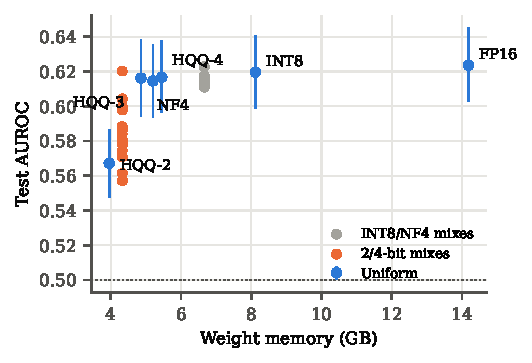
\includegraphics[width=\columnwidth]{figures/pareto.pdf}
\caption{Memory vs.\ test AUROC, Qwen-7B on cleaned Juliet. Uniform formats with 95\% CI. Uniform 3- and 4-bit match FP16; INT8/NF4 mixtures (grey) cost more memory than NF4 for no gain; at 2 bits, layer choice (orange) spans 0.06 AUROC at constant memory.}
\label{fig:pareto}
\end{figure}

\begin{table}[t]
\centering
\caption{Qwen2.5-Coder-3B on PrimeVul unpaired test (937 functions).}
\label{tab:pv}
\begin{tabular}{lrcc}
\toprule
Config & Mem.\,(GB) & AUROC & $\Delta$AUROC [95\% CI] \\
\midrule
FP16 & 5.75 & 0.666 & -- \\
INT8 & 3.21 & 0.673 & +0.007 [$-$0.001, 0.015] \\
NF4  & 1.91 & 0.659 & $-$0.007 [$-$0.017, 0.003] \\
top-$\stask$ (18/18) & 2.56 & 0.657 & $-$0.009 [$-$0.019, 0.000] \\
HQQ-4 & 2.03 & 0.683 & +0.016 [0.003, 0.029] \\
HQQ-3$^\ast$ & 1.79 & 0.304 & $-$0.362 [$-$0.415, $-$0.311] \\
HQQ-2$^\ast$ & 1.39 & 0.457 & $-$0.210 [$-$0.259, $-$0.157] \\
\bottomrule
\multicolumn{4}{l}{\footnotesize $^\ast$0\% YES/NO compliance: output has collapsed (Sec.~\ref{sec:collapse}).}
\end{tabular}
\end{table}

\begin{table}[t]
\centering
\caption{Qwen-3B, PrimeVul unpaired: 9 of 36 layers at HQQ-4, rest HQQ-2 (all 1.55\,GB). Compliance: share of functions whose top token is YES/NO.}
\label{tab:collapse}
\begin{tabular}{lcc}
\toprule
Layer selection & AUROC & Compliance \\
\midrule
FP16 reference & 0.666 & 99.9\% \\
top-$\sUp$ & 0.471 & 0\% \\
random, 8 seeds with 0\% compliance & 0.378--0.671 & 0\% \\
random s7 & 0.413 & 99.5\% \\
random s8 & 0.556 & 98.3\% \\
\bottomrule
\end{tabular}
\end{table}

\subsection{At 2 bits, layer choice is a lottery}\label{sec:twobit}
Uniform HQQ-2 loses 0.057 AUROC on Qwen-7B. Keeping 7 of 28 layers at 4 bits (about 0.4\,GB extra) gives very different outcomes at identical memory (Fig.~\ref{fig:lowbit}). Ten random layer sets reach $0.590 \pm 0.016$ (range 0.561--0.620; the best is within 0.004 of FP16). Layer choice is therefore consequential in this regime. The question is whether any sensitivity metric finds good sets better than chance.

\textbf{Depth-correlated metrics are harmful.} The $\sgen$ and $\slt$ profiles grow with depth (Spearman $\rho$ with layer index 0.73 for $\sgen$; $\slt$ is monotone, Fig.~\ref{fig:depth}). Top-$\sgen$ therefore selects exactly layers 21--27, identical to the last-7 control, and it is the worst configuration (0.557), \emph{below} uniform 2-bit.

\textbf{Task sensitivity is no better than random.} $\stask$ selects mostly middle layers (10, 11, 15, 17, 18, 26, 27) and reaches 0.598, above 6 of 10 random sets ($+0.5$ sd). Single-layer $\Delta$AUROC on calibration data is uncorrelated with $\stask$ ($\rho = 0.05$).

\textbf{Deployment-context sensitivity does not fix it.} A plausible explanation for $\stask$'s failure is context mismatch: it perturbs one layer while all others are FP16, whereas in deployment every other layer is 2-bit. $\sUp$ removes this mismatch by upgrading one layer at a time inside the uniform 2-bit model. It selects layers 0, 15--18, 26 and 27 and reaches only 0.571, below 9 of 10 random sets. The $\sUp$ profile explains why: upgrading a single layer to 4 bits \emph{increases} divergence from FP16 for 11 of 28 layers (20 of 36 on Qwen-3B), and $\sUp$ agrees only weakly with the same upgrade's effect on calibration AUROC ($\rho = 0.33$). Layer contributions at 2 bits are strongly non-additive, so no single-layer ranking can be expected to assemble a good set, whichever context it is measured in.

\textbf{Exploratory pattern.} Across the 15 budget-matched 2-bit configurations on Qwen-7B, AUROC correlates negatively with the number of protected layers among the last seven ($r = -0.55$) and positively with those among layers 14--19 ($r = 0.37$). With 15 configurations this is suggestive only. It is consistent with the failure of depth-correlated metrics, and suggests interaction-aware search (e.g.\ greedy or evolutionary) over random-but-structured candidates as future work.

\subsection{Model-size-dependent collapse and the compliance gate}\label{sec:collapse}
Qwen-3B collapses one bit earlier than Qwen-7B. At HQQ-3 and HQQ-2 it never emits YES or NO as its top token (Table~\ref{tab:pv}), whereas Qwen-7B stays fully compliant down to 2 bits. Once outputs have collapsed, the logit-ratio score no longer measures the task, and AUROC becomes arbitrary. Uniform HQQ-3 scores 0.304, below chance. The 2/4-bit mixes with 0\% compliance span 0.378--0.671, and one of them exceeds FP16 (Table~\ref{tab:collapse}). Only two of ten random sets stay compliant, and both are well below FP16 (0.413, 0.556). As with the FP16 floor effect, an evaluation that reported AUROC alone would draw arbitrary conclusions. We therefore add a second gate: any quantized configuration must also retain output compliance before its AUROC is interpreted.

\begin{figure}[t]
\centering
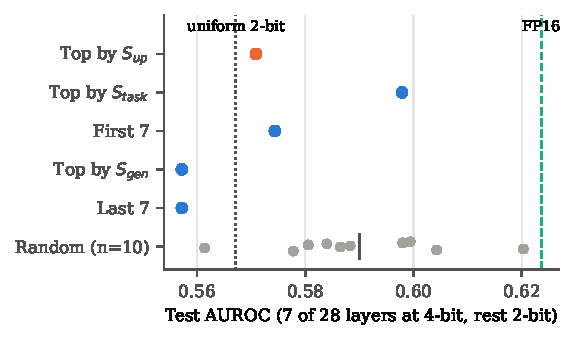
\includegraphics[width=\columnwidth]{figures/lowbit_selection.pdf}
\caption{2-bit operating point (Qwen-7B, cleaned Juliet): 7 layers at HQQ-4, rest HQQ-2 (all $\approx$4.43\,GB). Grey: 10 random layer sets (bar: mean). No sensitivity metric beats the random distribution; depth-correlated $\sgen$ coincides with the last-7 control and is worst, and deployment-context $\sUp$ is below 9 of 10 random sets.}
\label{fig:lowbit}
\end{figure}

\begin{figure*}[t]
\centering
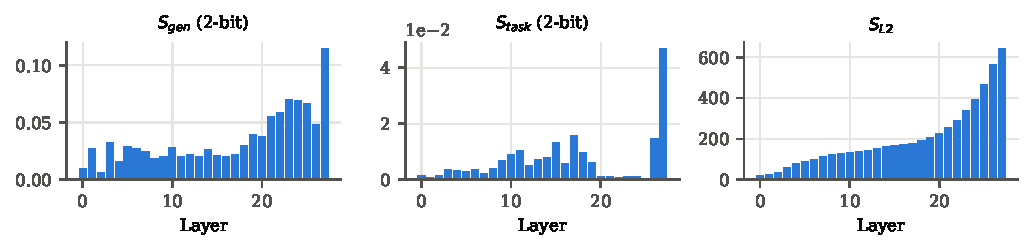
\includegraphics[width=0.85\textwidth]{figures/sensitivity_depth.pdf}
\caption{Per-layer sensitivity of Qwen-7B (calibration split). $\sgen$ and $\slt$ grow with depth, so ranking by them protects the last layers; $\stask$ peaks in the middle layers and at the final layer.}
\label{fig:depth}
\end{figure*}

\subsection{Quantization shifts calibration more than ranking}\label{sec:calib}
Fig.~\ref{fig:shift} shows $P(\text{vuln})$ distributions. HQQ-2 compresses both classes into 0.5--0.9 (mean 0.70 vs 0.49 in FP16), while its AUROC drops only to 0.567. At the FP16 threshold for 90\% recall, every 2-bit configuration flags all code (FPR 1.0). NF4 shifts scores downward and misses 35 vulnerable functions that FP16 caught at that threshold, though its AUROC is equivalent. On PrimeVul, NF4 raises F1 at a 0.5 threshold from 0.20 to 0.47 with no change in AUROC. Fixed-threshold metrics (accuracy, F1, recall at 0.5) therefore conflate calibration with detection ability. For deployment, the threshold must be re-selected on calibration data for each quantized model. This is cheap, but it is routinely omitted.

\begin{figure}[t]
\centering
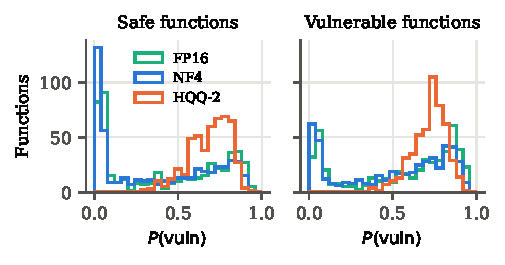
\includegraphics[width=\columnwidth]{figures/score_shift.pdf}
\caption{Distribution of $P(\text{vuln})$ for Qwen-7B on cleaned Juliet test. NF4 tracks FP16; HQQ-2 collapses both classes towards 0.5--0.9.}
\label{fig:shift}
\end{figure}

\subsection{Other observations}
\textbf{Context-aware pruning.} Removing comments before scoring (the CAP component of the original framework) has no effect on sanitised code ($-0.006$ vs $-0.009$ without), since the sanitiser already strips comments. On raw benchmarks, comments carry label cues, which likely explains CAP's apparent benefit in the prototype.
\textbf{Latency.} On T4, FP16 is fastest (0.18\,s per function, median). Quantization trades speed for memory: NF4 0.37\,s, and HQQ 0.77--1.07\,s with its PyTorch backend.

%=====================================================================
\section{Discussion and Limitations}
%=====================================================================
\textbf{Practical guidance.} (1) Gate on FP16 signal with CIs before comparing compressed models. (2) Never evaluate on unsanitised Juliet. (3) Use uniform 4-bit (or 3-bit) quantization; it is equivalent to FP16 and mixed INT8/NF4 is not worth its memory. (4) Check output compliance for every configuration; a collapsed model's AUROC is meaningless, and smaller models collapse at higher bit-widths. (5) Below 4 bits, layer allocation matters but is not predicted by single-layer sensitivity. Do not rank layers by depth-correlated metrics, and always compare any allocation method against a multi-seed random baseline. (6) Report threshold-free metrics, and re-calibrate thresholds after quantization.

\textbf{Limitations.} Absolute detection performance is modest (AUROC 0.62--0.67), consistent with prior findings that LLMs struggle with realistic vulnerability detection~\cite{ding2024primevul,ullah2024secllmholmes}. Our conclusions concern relative degradation, and may differ for stronger or fine-tuned detectors. We use weight-only, calibration-free or calibration-light quantization (bitsandbytes, HQQ). GPTQ/AWQ~\cite{frantar2023gptq,lin2024awq} may behave differently at 2--3 bits. Only two model/dataset settings pass the gate. Juliet is synthetic, and PrimeVul labels contain noise. Function-level classification ignores interprocedural context. Our sanitiser removes known lexical cues; residual structural cues in Juliet's templates may remain.

\textbf{Future work.} Fine-tuning (e.g.\ QLoRA~\cite{dettmers2023qlora}) to raise FP16 signal before compression; calibration-based 2--3-bit methods; interaction-aware layer allocation (greedy, evolutionary or learned) evaluated against random baselines; and larger calibration sets, since our 200-function calibration split limits how finely layer effects can be resolved.

%=====================================================================
\section{Conclusion}
%=====================================================================
For LLM-based vulnerability detection, the most consequential decisions in a quantization study come before quantization: whether the FP16 model has signal, and whether the benchmark leaks its labels. Where both checks pass, uniform 4-bit and 3-bit quantization preserve detection ability at roughly a third of FP16 memory, and sensitivity-guided mixing adds nothing. Below that, models collapse at a size-dependent bit-width, and output compliance must be checked before AUROC means anything. At 2 bits layer allocation matters, but neither existing sensitivity metrics nor a deployment-context variant beat random selection, because layer effects are non-additive. Mixed precision for this task therefore needs interaction-aware search, not better single-layer scores.

\section*{Artifact Availability}
Code, sanitised splits, configurations and all per-function predictions: \pending{GitHub URL}.

\bibliographystyle{IEEEtran}
\bibliography{refs}

\end{document}
